\scanpage{293}
\uline{\unsure{Cor}})

Les foncteurs $i_N,\tau_N$ commutent à \unsure{ttes|toutes} les sortes de limites inductives et projectives, $q_N$ commute aux $\underset{\longrightarrow}{\lim}$, $\varphi_N$ aux $\underset{\longleftarrow}{\lim}$.

Les foncteurs $i_N,\varphi_N$ sont pl. fid., les foncteurs $q_N,\tau_N$ sont des foncteurs localisation. \deleted{\unsure{Comme}} Pour $\tau_N$ (puisque il est exact, et commute aux $\underset{\longrightarrow}{\lim}$ et $\underset{\longleftarrow}{\lim}$) c'est la localisation mod une sous-cat. abélienne épaisse, stable par $\underset{\longrightarrow}{\lim}$ et $\underset{\longleftarrow}{\lim}$; en fait, c'est précisément la sous-cat $\mathcal M^{N-1}$ (qui est ainsi décrite \deleted{\unsure{ici}} en termes de $\mathcal M_N$).

\margin{\figure{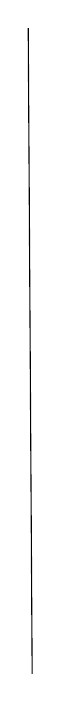
\begin{tikzpicture}\draw (0,0)--(-.05,8.2);\end{tikzpicture}}}
\margin{294}
